\documentclass[
    coverwidth=14cm,
    coverheight=21cm,
    spinewidth=25mm,
    flapwidth=6cm,
    wrapwidth=5mm,
]{bookcover}

\usepackage{xeCJK}
\usepackage{fontspec}
\usepackage{graphicx}
\usepackage{tikz}
\usepackage{microtype}

\setCJKmainfont{Noto Serif CJK SC}
\setCJKsansfont{Noto Sans CJK SC}
\setCJKmonofont{Noto Sans Mono CJK SC}

\setCJKfamilyfont{song}{Noto Serif CJK SC}
\setCJKfamilyfont{hei}{Noto Sans CJK SC}
\setCJKfamilyfont{fs}{Noto Serif CJK SC}

\newcommand{\CJKrmfamily}{\CJKfamily{song}}
\newcommand{\CJKsansfamily}{\CJKfamily{hei}}

\definecolor{WarmWhite}{RGB}{250,252,245}
\definecolor{SpringGreen}{RGB}{170,220,170}


\newbookcovercomponenttype{center rotate}{
    \vfill
    \centering
    \rotatebox[origin=c]{-90}{#1}
    \vfill}

\begin{document}

\begin{bookcover}

\begin{bookcoverelement}{color}{bg whole}
    WarmWhite
\end{bookcoverelement}

% 前折页、后折页背景颜色渐变
\begin{bookcoverelement}{tikz}{bg whole}
\shade[top color=SpringGreen!40,
       bottom color=WarmWhite]
       (0,0) rectangle (\partwidth,\partheight);
\end{bookcoverelement}

% 前封面、书脊、后封面统一背景图
\begin{bookcoverelement}{picture}{bg whole without flaps}
./figures/covers/background.jpeg
\end{bookcoverelement}

% 前封面图片
% \begin{bookcoverelement}{center}{front}
% 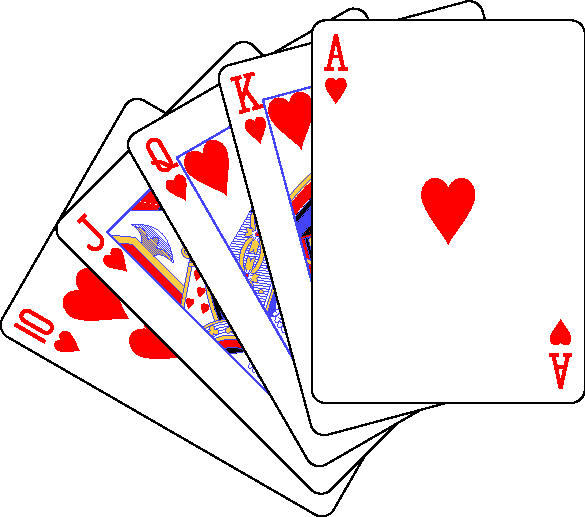
\includegraphics[width=0.8\partwidth]{./figures/bookcover-cards.pdf}
% \end{bookcoverelement}

% 前封面标题
\begin{bookcoverelement}{normal}{front}[3cm,4cm,3cm,5cm]

\end{bookcoverelement}

% 书脊

\begin{bookcoverelement}{center rotate}{spine}

\end{bookcoverelement}

% 后封面
\begin{bookcoverelement}{normal}{back}[2cm,2cm,2cm,2cm]

\end{bookcoverelement}

% 前折页
\begin{bookcoverelement}{normal}{front flap}[1cm,1cm,1cm,2cm]
\color{white}
作者简介：

作者长期从事人工智能与复杂系统研究，
关注策略学习与决策智能。

\vfill
\centering
% 
\includegraphics[width=3cm]{./figures/bookcover-dice.pdf}
\end{bookcoverelement}

% 后折页
\begin{bookcoverelement}{normal}{back flap}[1cm,2cm,1cm,2cm]

\end{bookcoverelement}

\end{bookcover}

\end{document}